\documentclass[a4paper,12pt]{article}
\usepackage[T1,T2A]{fontenc}
\usepackage[utf8]{inputenc}
\usepackage[english,ukrainian]{babel}


\usepackage{ upgreek }
\usepackage{amsmath}

\usepackage{graphicx}
\graphicspath{{./pictures/}}
\DeclareGraphicsExtensions{.pdf,.png,.jpg}

\usepackage[unicode=true,colorlinks=true,urlcolor=blue,citecolor=green,linkcolor=blue]{hyperref}
\usepackage[ukrainian,nameinlink]{cleveref}
\usepackage{geometry} % Меняем поля страницы
\geometry{left=2cm}% левое поле
\geometry{right=1.5cm}% правое поле
\geometry{top=1cm}% верхнее поле
\geometry{bottom=2cm}% нижнее поле



\begin{document}
	
	\begin{titlepage}
		\vspace*{6cm}
		\begin{center}
			
			\large
			\textbf{Звіт}\\
			\textbf{до лабораторної роботи №1:}\\
			\textbf{<<Чисельне моделювання для рівняння теплопровідності.>>}
			
		\end{center}
		
		\vspace{8cm}
		\begin{flushright}
			студента 1-го курсу магістратури\\
			факультету комп'ютерних наук та кібернетики\\
			Кравця Олексія
		\end{flushright}
		
	\end{titlepage}

\newpage
\tableofcontents
\newpage
\section{Постановка задачі}

Маємо наступне рівняння теплопровідності зі сталими коефіцієнтами

\begin{equation} \label{eq1}
	\frac{\partial \omega}{\partial t} = a \left( \frac{\partial^2 \omega}{\partial x^2} + \frac{\partial^2 \omega}{\partial y^2}\right) + f(x,y,t) 
\end{equation}

в наступній прямокутній області $[0,l_1]\times[0,l_2]$, $t \in (0,1)$.

Також даний тестовий розв'язок для варіанту 1:
\begin{equation} \label{eq2}
	\omega_{test}(x,y,t) = A e^{k_1 x + k_2 y + (k_1^2 + k_2^2) a t}
\end{equation}

Відновлюємо праву частину $f$ по відомому тестовому розв'язку (\ref{eq2}). Розпишемо це

\begin{displaymath}
	f(x,y,t) = \frac{\partial \omega_{test}}{\partial t} - a\left( \frac{\partial^2 \omega_{test}}{\partial x^2} + \frac{\partial^2 \omega_{test}}{\partial y^2}\right) = (k_1^2 + k_2^2)a A e^{(\cdots)} - a \left( k_1^2 A e^{(\cdots)} + k_2^2 A e^{(\cdots)} \right) =0
\end{displaymath}

Розглядаємо задачу з першими крайовими умовами.
\begin{equation} \label{eq3}
	\begin{aligned}
		&\omega(x,y,0) = \omega_{test}(x,y,0)	\\
		&\omega(0,y,t) = \omega_{test}(0,y,t)	\\
		&\omega(l_1,y,t) = \omega_{test}(l_1,y,t)	\\
		&\omega(x,0,t) = \omega_{test}(x,0,t)	\\
		&\omega(x,l_2,t) = \omega_{test}(x,l_2,t)	\\
	\end{aligned}
\end{equation}

\section{Опис методів}

\subsection{Явна різницева схема}

Позначимо $u$ наближений розв'язок, $h$ - крок по простору (спільний для $x,y$), $\tau$ - крок по часу. Тоді можемо так записати рівняння (\ref{eq1})

\begin{equation} \label{eq4}
	\frac{\partial u}{\partial t} = a \left( \frac{\partial^2 u}{\partial x^2} + \frac{\partial^2 u}{\partial y^2}\right) + f(x,y,t)
\end{equation}

Позначимо $x_k = kh$, $y_m = mh$, $t_\nu = \nu \tau$, $f_{km}^{\nu} = f(x_k, y_m, t_{\nu})$
\begin{equation}
	\begin{aligned}
		&\Lambda_1 u_{k,m}^{\nu}= \frac{ u_{k-1,m}^{\nu} - 2 u_{k,m}^{\nu} + u_{k+1, m}^{\nu} }{h^2} \\
		&\Lambda_2 u_{k,m}^{\nu} = \frac{ u_{k,m-1}^{\nu} - 2 u_{k,m}^{\nu} + u_{k, m+1}^{\nu} }{h^2} \\ 
		&\Lambda u_{k,m}^{\nu} = \Lambda_1 u_{k,m}^{\nu} + \Lambda_2 u_{k,m}^{\nu}
	\end{aligned} \nonumber
\end{equation}

Явна різницева схема має такий вигляд
\begin{equation} \label{eq5}
	\frac{u_{k,m}^{\nu} - u_{k,m}^{\nu -1}}{\tau} - a\Lambda u_{k,m}^{\nu-1} = f_{k,m}^{\nu-1}
\end{equation}

Ця схема стійка при $\tau \le h^2/4$.

\subsection{Метод змінних напрямків}

Позначення не змінилися.

Метод змінних напрямків складається з двох полукроків

\begin{align}
	&\frac{u_{k,m}^{\nu- 1/2} - u_{k,m}^{\nu -1}}{\tau/2} - a \Lambda_1 u_{k,m}^{\nu -1/2} - a \Lambda_2 u_{k,m}^{\nu-1} = f_{k,m}^{\nu- 1/2} \label{eq6} \\
	&\frac{u_{k,m}^{\nu} - u_{k,m}^{\nu -1/2}}{\tau/2} - a \Lambda_1 u_{k,m}^{\nu -1/2} - a \Lambda_2 u_{k,m}^{\nu} = f_{k,m}^{\nu} \label{eq7}
\end{align}

Рівняння (\ref{eq6}), (\ref{eq7}) можна переписати у вигляді, що дозволяє використати метод прогонки. Розпишемо рівняння (\ref{eq6})

\begin{equation}
	\begin{aligned}
		&\frac{a \tau}{2 h^2} u_{k-1,m}^{\nu - 1/2} - \left( 1 + \frac{a \tau}{h^2} \right) u_{k,m}^{\nu -1/2} + \frac{a \tau}{2h^2} u_{k+1,m}^{\nu -1/2} = F_{k,m}^{\nu -1/2}, \quad \text{де} \\
		&F_{k,m}^{\nu -1/2} = \frac{\tau}{2} \left( -a\Lambda_2 u_{k,m}^{\nu -1} -f_{k,m}^{\nu- 1/2} \right) - u_{k,m}^{\nu -1}
	\end{aligned} \nonumber
\end{equation}

Отже для кожного фіксованого $m$ маємо систему лінійних алгебраїчних рівнянь, що можна вирішити методом прогонки.

Розпишемо рівняння (\ref{eq7})

\begin{equation}
	\begin{aligned}
		&\frac{a \tau}{2 h^2} u_{k,m-1}^{\nu} - \left( 1 + \frac{a \tau}{h^2} \right) u_{k,m}^{\nu} + \frac{a \tau}{2h^2} u_{k,m+1}^{\nu} = F_{k,m}^{\nu}, \quad \text{де} \\
		&F_{k,m}^{\nu} = \frac{\tau}{2} \left( -a\Lambda_1 u_{k,m}^{\nu -1/2} -f_{k,m}^{\nu- 1/2} \right) - u_{k,m}^{\nu -1/2}
	\end{aligned} \nonumber
\end{equation}

Ця схема абсолютна стійка.

\subsection{Двокроковий симетризований алгоритм}

Позначення не змінилися. Додамо позначення $c$ - кількість пройдених алгоритмом кроків.

Візьмемо точки $u_{k,m}$, що задовольняють умові: $(k+u+c)$ ділиться на 2. Будемо оновлювати їх за явної різницевою схемою.

\begin{equation} \label{eq8}
	\frac{u_{k,m}^{\nu} - u_{k,m}^{\nu -1}}{\tau} - a\Lambda u_{k,m}^{\nu-1} = f_{k,m}^{\nu-1}
\end{equation}

Після цього розглянемо точки, що залишилися, вони задовольняють умові: $(k+u+c)$ не ділиться на 2. Будемо оновлювати їх за неявно різницевою схемою, завдяки рівнянню (\ref{eq8}) можна буде явним чином отримати $u_{k,m}^{\nu}$.

\begin{equation} \label{eq9}
		\frac{u_{k,m}^{\nu} - u_{k,m}^{\nu-1}}{\tau} - a\Lambda u_{k,m}^{\nu} = f_{k,m}^{\nu}
\end{equation}

Розпишемо рівняння (\ref{eq9}), що отримати $u_{k,m}^{\nu}$ явним чином.

\begin{displaymath} 
	u_{k,m}^{\nu} = \left( f_{k,m}^{\nu} + \frac{u_{k,m}^{\nu -1}}{\tau} + a \left( \frac{u_{k-1,m}^{\nu} + u_{k+1,m}^{\nu}}{h^2} \right) + a \left( \frac{u_{k,m-1}^{\nu} + u_{k,m+1}^{\nu}}{h^2} \right) \right) \frac{\tau h^2}{h^2 + 4 a \tau}
\end{displaymath}

Ця схема абсолютна стійка, та більш точна на парних часових кроках.

\section{Результати}

Розглядаємо задачу в області $[0,1] \times [0,1]$, початковий час $t_0 = 0$. Просторовий крок $h = 0.1$, часовий крок $\tau = h**2/4$ для збіжності явної схеми. 

Параметри для рівняння (\ref{eq1}), (\ref{eq2}) рівні 1, крім $a= 0.1$.


\begin{figure}[h]
	\center{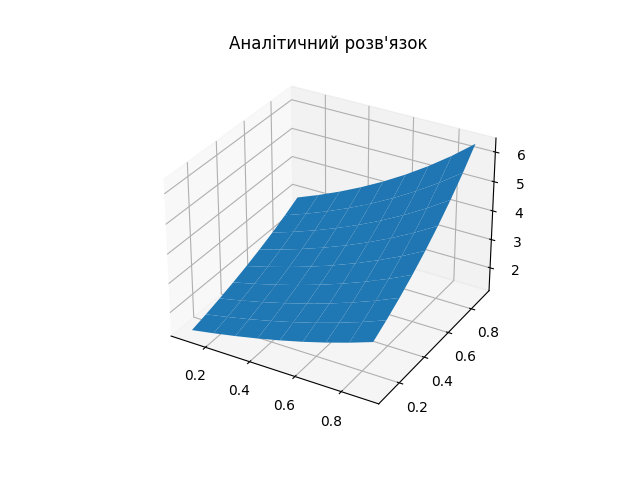
\includegraphics[width=1\linewidth]{Figure1.png}}
	\caption{Рисунок аналітичного розв'язку на 100 часовому кроці.}
	\label{ris1}
\end{figure}

На рисунку (\ref{ris2}) позначені методи:
\begin{itemize}
	\item \textit{method1} - Явна різницева схема;
	\item \textit{method2} - Метод змінних напрямків;
	\item \textit{method3} - Двокроковий симетризований алгоритм.
\end{itemize}

\newpage
\begin{figure}[ht]
	\center{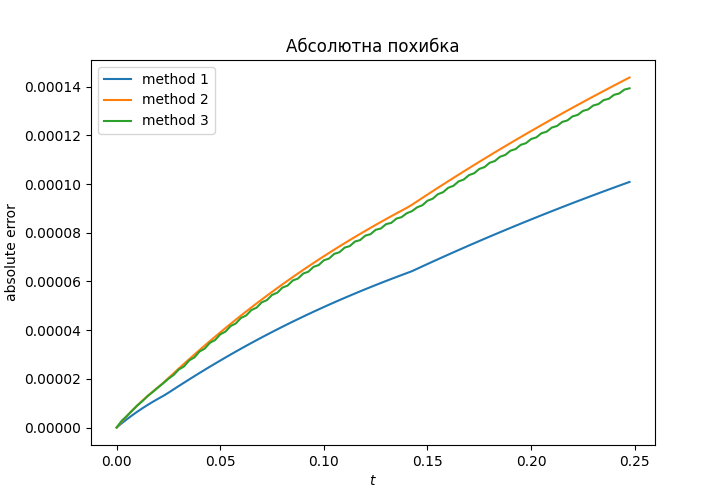
\includegraphics[width=1\linewidth]{Figure2.png}}
	\caption{Графіки абсолютної помилки}
	\label{ris2}
\end{figure}

На 100 часовому кроці маємо такі значення абсолютної похибки:
\begin{itemize}
	\item Явна різницева схема - $e = 1E^{-4}$;
	\item Метод змінних напрямків - $e = 1.4E^{-4}$;
	\item Двокроковий симетризований алгоритм - $e = 1.4E^{-4}$.
\end{itemize}


\newpage
\section{Висновки}

Ми реалізували та провели тести трьох методів чисельного моделювання. На тестах видна залежність двокрокового симетризованого алгоритму від парності часового кроку.

\addcontentsline{toc}{section}{Література}
\begin{thebibliography}{}
	\bibitem{Volkov}  Е.А.Волков Численные методы, 1987, Москва <<Наука>>
	\bibitem{GR_Onockiy} Грищенко О.Ю., Оноцький В.В. Дисипативніть двокрокових симетризованих алгоритмів для гіперболічних рівнянь переносу, 2000, <<Вісник Київського університету>>
\end{thebibliography}

\end{document}